\documentclass[tikz,border=10pt]{standalone}
\begin{document}
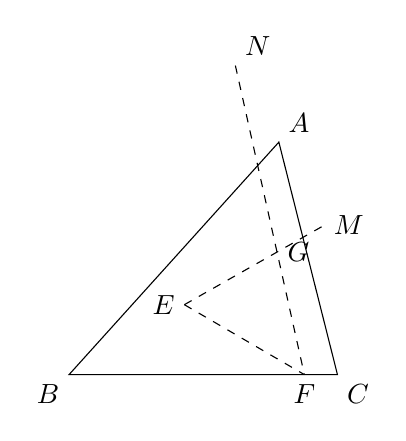
\begin{tikzpicture}[scale=1.2]
  % Points
  \coordinate (B) at (0,0);
  \coordinate (C) at (2.84,0);
  \coordinate (A) at (2.22,2.46);
  \coordinate (E) at (1.22,0.74);
  \coordinate (M) at (2.70,1.58);
  \coordinate (F) at (2.49,0);
  \coordinate (G) at (2.21,1.30);
  \coordinate (N) at (1.76,3.27);

  % Solid triangle
  \draw (B) -- (C) -- (A) -- cycle;

  % Dashed segments
  \draw[dashed] (N) -- (F);
  \draw[dashed] (E) -- (M);
  \draw[dashed] (E) -- (F);

  % Labels
  \node[above right] at (N) {$N$};
  \node[above right] at (A) {$A$};
  \node[right] at (M) {$M$};
  \node[left] at (E) {$E$};
  \node[below left] at (B) {$B$};
  \node[below right] at (C) {$C$};
  \node[below] at (F) {$F$};
  \node[right] at (G) {$G$};
\end{tikzpicture}
\end{document}
